\StartOf{Lecture 16}

\Today{(1) Received Power Models, (2) Noise Energy, (3) Link Budgeting}

\announcements{
\begin{itemize}
  \item Today's reading: Rice 6.4.  
\end{itemize}
}

\section{Noise and Received Power Models}

This section starts to make the connection between the energy per bit which we use in probability of error formulas to the transmit power and distance between the transmitter and receiver in a given communication system.  Given that we want our wireless communication system to operate in some application or for some link, how can we calculate how much power will be received, typically?  We do this here for both wireless and wired channels.  Wireless channels we divide into free space channels, and obstructed (non-free-space channels).  My research and experience is in the design of wireless systems, so I must warn you that I provide much more detail for wireless than for wired communication systems.

\subsection{Free Space}

`Free space' is the idealization in which nothing exists except for
the transmitter and receiver, and can really only be used for deep space
communications.  But, this formula serves as a starting point for other
radio propagation formulas.  In free space, the received power is calculated from
the Friis formula,
\[
C = P_R = P_T G_T G_R \left(\frac{ \lambda}{4\pi R_0}\right)^2 
\left( \frac{ R_0}{R}\right)^2
\]
where
\begin{itemize}
  \item $G_T$ and $G_R$ are the antenna gains at the transmitter and
  receiver, respectively.
  \item $P_T$ is the transmit power.
  \item $\lambda$ is the wavelength at signal frequency.
  For narrowband signals, the wavelength is nearly constant across
  the bandwidth, so we just use the center frequency $f_c$.  Note
  that $\lambda = c / f_c$ where $c = 3\times 10^8$ meters per
  second is the speed of light.
  \item $R_0$ is a reference distance, say 1 meter or 10 meters. You may notice that the $R_0$s cancel, so why have I put it in?  It is useful for understanding the relationships and for keeping track of the units. 1) One can measure the received power at a reference distance $R_0$ during testing, and then replace the $P_T G_T G_R \left(\frac{ \lambda}{4\pi R_0}\right)^2$ part with the measurement; 2) Each fraction has units that cancel; and 3) We consider the $\left( \frac{ R_0}{R}\right)^2$ part as the \emph{path loss}, i.e., loss due to the actual path length (distance between the transmitter and receiver).
\end{itemize}
Here, everything is in linear terms.  Typically people use decibels
to express these numbers, and we will write $\dBm{P_R}$ or
$\dB{G_T}$ to denote that they are given by:
\begin{eqnarray}
  \dBm{P_R}  &=& 10 \log_{10} P_R \nnn
  \dB{G_T} &=& 10 \log_{10} G_T \nnn
\end{eqnarray}

The Friis formula, given in dB, is
\begin{equation} \label{E:FriisIndB}
 \dBm{C} = \dB{G_T} + \dB{G_R}  + \dBm{P_T} + 20 \log_{10} \frac{\lambda}{4\pi R_0} - 20 \log_{10} \frac{R}{R_0} 
\end{equation}
This says the received power, $C$, is linearly proportional to the log of the distance $R$.  

The received power at the reference distance $R_0$ is called $\dBm{P_0}$ and is given by:
\begin{equation} \label{E:P0_formula}
 \dBm{P_0} = \dB{G_T} + \dB{G_R}  + \dBm{P_T} + 20 \log_{10} \frac{\lambda}{4\pi R_0}
\end{equation}
Again, $\dBm{P_0}$  is something you might measure with a well-calibrated receiver and an antenna.  If you know (or estimate) $\dBm{P_0}$, then the relationship of received power (dBm) with distance $R$ is simply:
\begin{equation} \label{E:FriisIndBSimple}
 \dBm{C} = \dBm{P_0} - 20 \log_{10} \frac{R}{R_0} .
\end{equation}


%The Rice book writes the Friis formula as
%\[
% \dBm{C} = \dB{G_T} + \dB{G_R}  + \dBm{P_T} + \dB{L_p}
%\]
%where 
%\[
% \dB{L_p} = + 20 \log_{10} \frac{\lambda}{4\pi} - 20 \log_{10} R 
%\]
%where $\dB{L_p}$ is called the ``channel loss''.  (This name that Rice chose is unfortunate because if it was positive, it would be a ``gain'', but it is typically very negative.  My opinion is, it should be called ``channel gain'' and have a negative gain value.)

There are also typically other losses in a transmitter / receiver system; losses in a cable, other imperfections, etc.  In the Rice book, these are labelled as $L$[dB]. You must subtract the dB loss from the left-hand side of (\ref{E:FriisIndB}):
\begin{equation} \label{E:FriisIndBSimpleLoss}
 \dBm{C} = \dBm{P_0} - 20 \log_{10} \frac{R}{R_0} -\dB{L}.
\end{equation}
Note that you need to be careful (because Rice is not) that if you call it a dB ``loss'', it is positive value that you subtract from (\ref{E:FriisIndBSimple}), but you if you call it a ``gain'' than it must be subtracted from (\ref{E:FriisIndBSimple}).



\subsection{Non-free-space Channels}

We don't study radio propagation path loss formulas in this course.  But, a very short summary is that radio propagation on Earth is different than the Friis formula suggests. Lots of other formulas exist that approximate the received power as a function of distance, antenna heights, type of environment, etc.  The main problem is that walls, trees, buildings, and terrain decrease the power that would be received as compared to the Friis model.  This is called ``shadowing'' in analogy to how objects shadow light.

The most common model for real world shadowing effects is the path loss exponent model, in which received power (dBm) is linear with the log of distance,
\begin{equation} \label{E:PLExponentModel}
  \dBm{C} = \dBm{P_0} - 10n_p \log_{10}\frac{R}{R_0},
\end{equation}
for some constant $n_p$. Here, $\dBm{P_0}$ is typically the same as we described earlier, that is, the path loss that the Friis model would predict at some short distance $R_0$ from the antenna.  Usually $R_0$ is a very short distance, like $1$ m or $10$ m. Effectively, because of shadowing caused by buildings, trees,
etc., the average loss may increase more quickly than $1/R^2$, instead, it may be more like $1/R^{n_p}$.  

Equivalently, in linear terms:
\[
C = P_R = P_T G_T G_R \left(\frac{ \lambda}{4\pi R_0}\right)^2 
\left( \frac{ R_0}{R}\right)^{n_p}
\]


This is a model that comes with lots of evidence from empirical measurement studies.  In dense urban areas like Manhattan, people observe a much higher $n_p$ than in rural areas.  In mountainous areas, we typically observe a higher $n_p$ than in flat areas.  When the antennas are both close to the ground, the $n_p$ is higher than when the antennas are held tens of meters away from the ground.  Finally, in buildings, we observe a higher $n_p$ when the walls are made of bricks or concrete, than when the walls are drywall and wood frame.  The value of $n_p$ may range from 2 to 4.5, with some values going lower than 2 or higher than 4.5.  In real life, you would want to measure $n_p$ in the type of environment you want to have your link operate in, or use values from the literature on measurement-based path loss models.

However, note that (\ref{E:PLExponentModel}) is only the \emph{average} received power.  In reality, any one particular measurement of received power a distance $R$ from the transmitter may be off by 10-30 dB from the average, due to differences in the particular path that the signal travels, due to small-scale fading, and for other reasons.


\subsection{Wired Channels}

Typically wired channels are lossy as well, but the loss is modeled as linear in the length of the cable.  For example, 
\[
 \dBm{C} = \dBm{P_T} - R (\dB{L_{1m}})
\]
where $P_T$ is the transmit power and $R$ is the cable length in meters, and $L_{1m}$ is the loss per meter.  


\subsection{Noise Energy}

The noise energy $N_0$ can be calculated as:
\[
N_0 = kT_{eq}
\]
where $k = 1.38 \times 10^{-23}$ J/K is Boltzmann's constant and $T_{eq}$ is
called the equivalent noise temperature in Kelvin.  This is a topic covered in
another course, and so you are not responsible for that material
here.  But in short, the equivalent temperature is a function of the receiver design, and $T_0$, the temperature of the environment at which the antenna is receiving from.  
$T_{eq}$ is always going to be higher than $T_0$.  Basically, all receiver circuits add
noise to the received signal.  With proper design (and more expensive and power-hungry components), $T_{eq}$ can be kept low.  






\section{System Design}
This section makes connections between the modulation performance formulas we've already discussed to the received power models just mentioned, in order to analyze a system design. 

For example, we may want to figure out what modulation, bit rate, and transmit power to use for a deep space communication system.  Or for a new long-range IoT system.  Or for a fiber-optic communications system.  You may find that you need several missing (or forgotten) connections to other topics in order to design a real-world communication system.  This lecture and the next lecture are designed to present these connections. 

As a digital communication system designer, your mission (if you choose to accept it) is to achieve:
\begin{enumerate}
 \item High data rate
 \item High fidelity (low bit error rate)
 \item Low transmit power 
 \item Low bandwidth
 \item Low transmitter/receiver complexity
 \item Long range
\end{enumerate}
But this is truly a mission impossible, because you can't have everything at the same time.  So the system design depends on what the desired system really needs and what are the acceptable trade-offs.  Typically some subset of requirements are given; for example, given the bandwidth limits, the received signal power and noise power, and bit error rate limit, what data rate can be achieved?  Using which modulation?

\section{Using the Relationship Flow Chart}

For a typical system design question, we are given some constraints (at the given limits) and asked to determine other system parameters.  For these types of problems I find it helpful to use the flow chart in Figure \ref{F:RelationshipsFlowChart} to keep track of my given constraints, the many functional relationships that exist in wireless communication system design, and thus how to get to the parameter of interest.  

In this lecture, we discuss this procedure, and define each of the variables we see in Figure \ref{F:RelationshipsFlowChart}, and to what they are related.  This lecture is about system design, and it cuts across electrical and computer engineering classes; in particular circuits, radio propagation, antennas, optics, and the material from this class.  You are expected to apply what you have learned in other classes (or learn the functional relationships that we describe here).

\begin{figure}[htbp]
    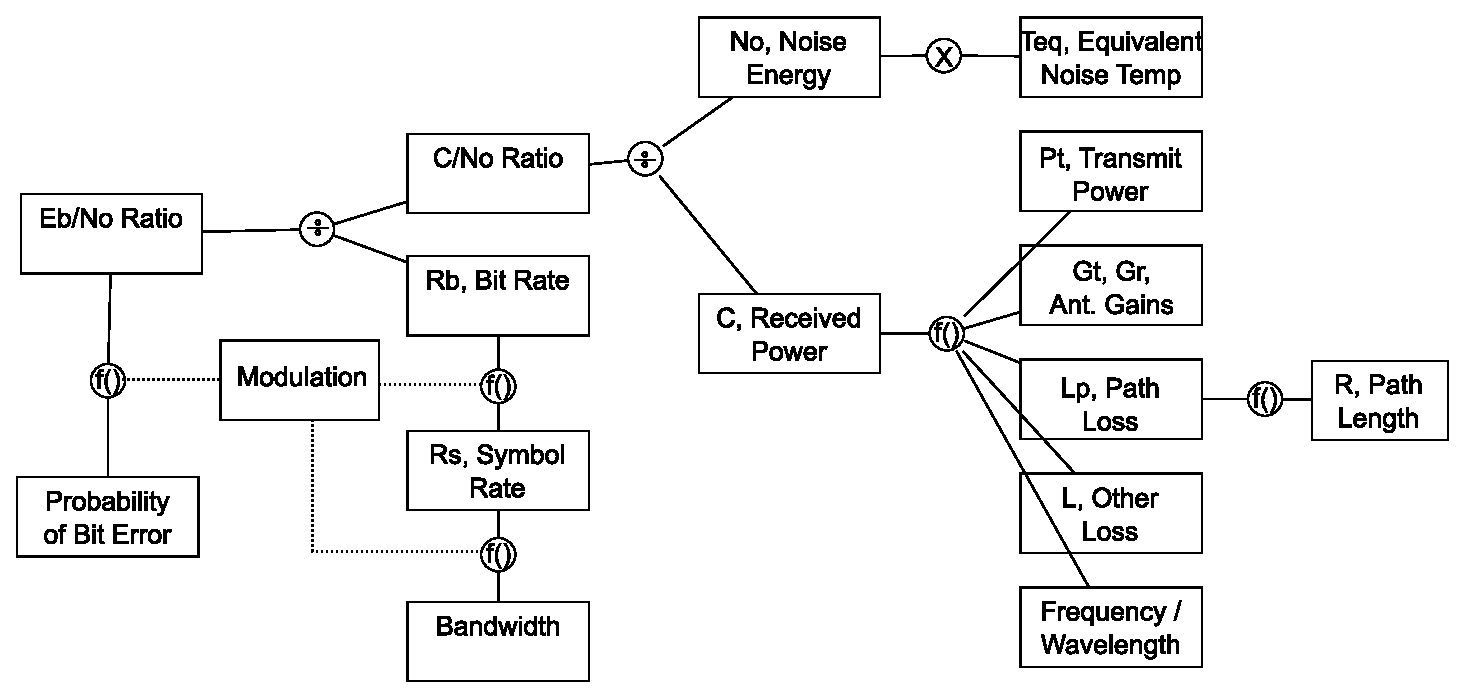
\includegraphics[width=6.5in]{../images/relationshipGraphDigiComm.eps}
    \caption{Relationships between important system design variables (rectangular boxes).  Functional relationships between variables are given as circles, with   division ($\div$), multiplication ($\times$), or another more complicated function $f()$. For example, $C/N_0$ is shown to have a divide by relationship with $C$ and $N_0$.  The effect of the choice of modulation impacts several functional relationships, \eg, the relationship between probability of bit error and $\Ebno$, which is drawn as a dotted line.}
    \label{F:RelationshipsFlowChart}
\end{figure}

\subsection{Link Budgets Given $C/N_0$}

The received power is denoted $C$, it has units of Watts.  What is $C/N_0$?  It is received power divided by noise energy.  It is a nebulous quantity, but it summarizes what we need to know about the signal and the noise for the purposes of system design.  
\begin{itemize}
%
 \item We (and other books) often describe both the received power as $P_R$, but in the Rice book it is typically denoted $C$.
%
 \item We know the probability of bit error is typically written as a function of $\Ebno$.  The noise energy is $N_0$.  The bit energy is $\En_b$.  We can write $\En_b = C T_b$, since energy is power $\times$ time.
To separate the effect of $T_b$, we often denote:
\[
  \Ebno = \frac{C}{N_0} T_b = \frac{C/N_0}{R_b}
\]
where $R_b = 1/T_b$ is the bit rate.  In other words, $C/N_0 = \Ebno   R_b$   What are the units of $C/N_0$? {\it Answer: Hz, 1/s}.  
 \item Note that people often report $C/N_0$ in dB Hz, which is
  \[
    10 \log_{10} \frac{C}{N_0}
  \]
%
 \item Be careful of Bytes (B) per second vs bits (b) per second.  Commonly, computer science 
people use Bps (kBps or MBps) when describing data rate.  For
example, if it takes 5 seconds to transfer a 1MB file, then software
often reports that the data rate is $1/5=0.2$ MBps or 200 kBps. But
the bit rate is $8/5$ Mbps or $1.6\times 10^6$ bps.  This number is $8\times$ larger so it is the one used by your ISP when selling you your internet service!
%
\end{itemize}

Given $C/N_0$, we can now relate bit error rate, modulation, bit rate, and bandwidth.

\Note{  
 We typically use $\Q{\cdot}$ and $\Qinv{\cdot}$ to relate BER and $\Ebno$ in each direction.  
 While you have Matlab, this is easy to calculate.  If you can program it into your 
 calculator, great.  Otherwise, it's really not a big deal to pull it 
 off of a chart or table.  For your convenience, the following tables/plots 
 of $\Qinv{x}$ will appear on Exam 2.  I am not picky about getting lots 
 of correct decimal places.}

\newpage
\centerline{ TABLE OF THE $\Qinv{\cdot}$ FUNCTION: }
\begin{tabular}{|l|l|l|}
  \hline
$\Qinv{1\times 10^{-6}} =  4.7534$ & $\Qinv{1\times 10^{-4}} =  3.719$ & $\Qinv{1\times 10^{-2}} =  2.3263$ \\
$\Qinv{1.5\times 10^{-6}} =  4.6708$ & $\Qinv{1.5\times 10^{-4}} =  3.6153$ & $\Qinv{1.5\times 10^{-2}} =  2.1701$ \\
$\Qinv{2\times 10^{-6}} =  4.6114$ & $\Qinv{2\times 10^{-4}} =  3.5401$ & $\Qinv{2\times 10^{-2}} =  2.0537$ \\
$\Qinv{3\times 10^{-6}} =  4.5264$ & $\Qinv{3\times 10^{-4}} =  3.4316$ & $\Qinv{3\times 10^{-2}} =  1.8808$ \\
$\Qinv{4\times 10^{-6}} =  4.4652$ & $\Qinv{4\times 10^{-4}} =  3.3528$ & $\Qinv{4\times 10^{-2}} =  1.7507$ \\
$\Qinv{5\times 10^{-6}} =  4.4172$ & $\Qinv{5\times 10^{-4}} =  3.2905$ & $\Qinv{5\times 10^{-2}} =  1.6449$ \\
$\Qinv{6\times 10^{-6}} =  4.3776$ & $\Qinv{6\times 10^{-4}} =  3.2389$ & $\Qinv{6\times 10^{-2}} =  1.5548$ \\
$\Qinv{7\times 10^{-6}} =  4.3439$ & $\Qinv{7\times 10^{-4}} =  3.1947$ & $\Qinv{7\times 10^{-2}} =  1.4758$ \\
$\Qinv{8\times 10^{-6}} =  4.3145$ & $\Qinv{8\times 10^{-4}} =  3.1559$ & $\Qinv{8\times 10^{-2}} =  1.4051$ \\
$\Qinv{9\times 10^{-6}} =  4.2884$ & $\Qinv{9\times 10^{-4}} =  3.1214$ & $\Qinv{9\times 10^{-2}} =  1.3408$ \\
\hline
$\Qinv{1\times 10^{-5}} =  4.2649$ & $\Qinv{1\times 10^{-3}} =  3.0902$ & $\Qinv{1\times 10^{-1}} =  1.2816$ \\
$\Qinv{1.5\times 10^{-5}} =  4.1735$ & $\Qinv{1.5\times 10^{-3}} =  2.9677$ & $\Qinv{1.5\times 10^{-1}} =  1.0364$ \\
$\Qinv{2\times 10^{-5}} =  4.1075$ & $\Qinv{2\times 10^{-3}} =  2.8782$ & $\Qinv{2\times 10^{-1}} =  0.84162$ \\
$\Qinv{3\times 10^{-5}} =  4.0128$ & $\Qinv{3\times 10^{-3}} =  2.7478$ & $\Qinv{3\times 10^{-1}} =  0.5244$ \\
$\Qinv{4\times 10^{-5}} =  3.9444$ & $\Qinv{4\times 10^{-3}} =  2.6521$ & $\Qinv{4\times 10^{-1}} =  0.25335$ \\
$\Qinv{5\times 10^{-5}} =  3.8906$ & $\Qinv{5\times 10^{-3}} =  2.5758$ & $\Qinv{5\times 10^{-1}} =  0$ \\
$\Qinv{6\times 10^{-5}} =  3.8461$ & $\Qinv{6\times 10^{-3}} =  2.5121$ &  \\
$\Qinv{7\times 10^{-5}} =  3.8082$ & $\Qinv{7\times 10^{-3}} =  2.4573$ &  \\
$\Qinv{8\times 10^{-5}} =  3.775$ & $\Qinv{8\times 10^{-3}} =  2.4089$ &  \\
$\Qinv{9\times 10^{-5}} =  3.7455$ & $\Qinv{9\times 10^{-3}} =  2.3656$ &  \\
\hline
\end{tabular}


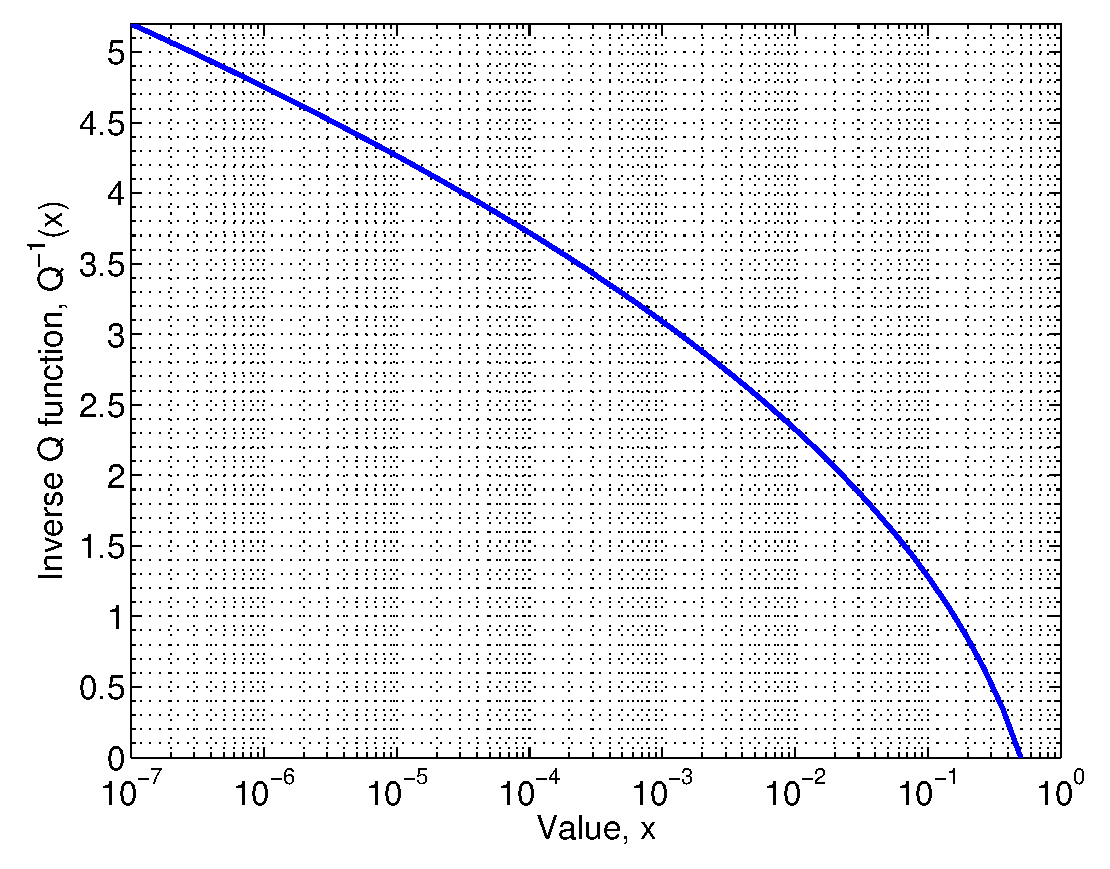
\includegraphics[width=5.5in]{../images/plotQinv.eps}






\subsection{Examples}

\Example{Rice 6.36}  

Consider a ``point-to-point'' microwave link. (Such links provide the internet backbone for cellular base stations and internet providers where fiber optic cables can't be installed, for example in rural areas.) Both antenna gains are 20 dB and the transmit antenna power is 10 W. The modulation is 51.84 Mbits/sec 256 square QAM with a carrier frequency of 4 GHz. Atmospheric losses are 2 dB and other incidental losses are 2 dB. A pigeon in the line-of-sight path causes an additional 2 dB loss. The receiver has an equivalent noise temperature of 400 K and an implementation loss of 1 dB. How far away can the two towers be if the bit error rate is not to exceed $10^{-8}$? Include the pigeon. 

Neal's hint: Use the dB version of Friis formula and subtract these mentioned dB losses: atmospheric losses, incidental losses, implementation loss, and the pigeon.

\Solution{
Starting with the modulation, $M=256$ square QAM ($\log_2 M = 8$, $\sqrt{M} = 16$), to achieve $\PR{\mbox{error}}=10^{-8}$,
\begin{eqnarray}
    10^{-8} &=& \frac{4}{\log_2 m} \frac{(\sqrt{M}-1)}{\sqrt{M}} \Q{\sqrt{\frac{3 \log_2 M}{M-1} \frac{\En_b}{N_0}}} 
  \nnn
    10^{-8} &=& \frac{4}{8} \frac{15}{16} \Q{\sqrt{\frac{3 (8)}{255} \frac{\En_b}{N_0}}} 
  \nnn
    10^{-8} &=& \frac{15}{32} \Q{\sqrt{\frac{24}{255} \frac{\En_b}{N_0}}} .
  \nnn
    \Ebno &=& \frac{255}{24} \left[ \Qinv{\frac{32}{15} 10^{-8} }\right]^2  = 319.0 \nn
\end{eqnarray}
The noise power $N_0 = kT_{eq} = 1.38\times 10^{-23} (\mbox{J/K}) 400   (\mbox{K}) = 5.52\times 10^{-21}$ J.  So 
$\En_b = 319.0 \times 5.52\times 10^{-21} = 1.76 \times 10^{-18}$ J.  Since $\En_b = C /R_b$ and the bit rate $R_b = 51.84 \times 10^6$ bits/sec,
$C = (51.84 \times 10^6) J (1.76 \times 10^{-18}) 1/sec = 9.13\times 10^{-11}$ W, or -100.4 dBW.

Switching to finding an expression for $C$, the wavelength is $\lambda = 3\times 10^8 \mbox{m/s} / 4\times 10^9 \mbox{1/s} = 0.075 m$, so:
\begin{eqnarray}
 \dBW{C} &=& \dB{G_T} + \dB{G_R}  + \dBW{P_T} + 20 \log_{10} \frac{\lambda}{4\pi} - 20 \log_{10} R - 2 \mbox{dB}- 2 \mbox{dB}- 2\mbox{dB} - 1\mbox{dB} 
   \nnn
         &=& 20 \mbox{dB} + 20 \mbox{dB} + 10 \mbox{dBW} + 20 \log_{10} \frac{0.075 m }{4\pi} - 20 \log_{10} R - 7 dB
   \nnn
         &=& -1.48 \mbox{dBW} - 20 \log_{10} R 
\end{eqnarray}
Plugging in $\dBm{C} = -100.4$ dBW $= -1.48 \mbox{dBW} - 20 \log_{10} R $ and solving for $R$,  we find $R = 88.3$ km.  Thus microwave towers should be placed at most 88.3 km (about 55 miles) apart.
}

